\documentclass{article}
\usepackage{amssymb,latexsym,amsmath,amsthm,mathrsfs}
\usepackage{graphicx}
\newtheorem{theorem}{Theorem}
\newtheorem{remark}[theorem]{Remark}
\newtheorem{conjecture}[theorem]{Conjecture}
\newtheorem{construction}[theorem]{Construction}
\newtheorem{lemma}[theorem]{Lemma}
\newtheorem{definition}[theorem]{Definition}
\newtheorem{corollary}[theorem]{Corollary}
\newcommand{\comment}[1]{}
\DeclareMathOperator{\Res}{Res}
\DeclareMathOperator{\ord}{ord}
\begin{document}
\title{Some fundamental results on modular forms}
\author{Jordan Bell}
%\keywords{}
%\subjclass[2000]{Primary: ; Secondary:  }
%\email{jbell3@connect.carleton.ca}
%\address{School of Mathematics and Statistics, Carleton
%University, 1125 Colonel By Drive, Ottawa, Ontario, K1S 5B6, Canada.}
\date{May 2, 2007}
\maketitle

\section{Introduction}
The purpose of this paper is to give complete proofs to several fundamental results about modular forms. Modular forms
are complex functions with certain analytic properties, and that transform nicely under a certain group of transformations
of the complex upper half plane. It turns out that modular forms can be used to study analytic number theory, by investigating
the coefficients in series expansions of the modular forms. In fact, often using
modular forms we can discover and prove things in number theory where a direct proof might not be obvious.
To help the reader get a feel for this, we will give an example; all the terms used here are defined in the paper.
An important class of modular forms, called Eisenstein series, have expansions that involve the divisor sum
$\sigma_r(n)=\sum_{d|n}d^r$. Another modular form, called the modular discriminant, has a series
expansion that involves the Ramanujan tau function, $\tau(n)$. Modular forms comprise vector spaces whose
dimensions we can explicitly determine. Using this  information one can prove
the congruence
\[
\tau(n) \equiv \sigma_{11}(n) \pmod{691}.
\]
We will develop all the results needed to prove this congruence and other similar
results (cf. \cite{MR938970}).

We have tried to find the clearest proofs in the literature for the results about modular forms in this paper.
The proofs use complex analysis and group theory, and do not assume advanced results.

In \S 2 we introduce a group action on the complex upper half plane, under which modular forms are well behaved.

Next in \S 3 we define modular forms and cusp forms, which are defined on the upper half plane.
We show that modular forms have Fourier expansions. Indeed it is often convenient to study a modular form through its
Fourier series. We also show that modular forms constitute complex vector spaces.
We explicitly construct 
a class of modular forms, namely the Eisenstein series, in \S 4. However, these are not cusp forms.
In \S 5 we construct a cusp form of weight 12,
and prove estimates on the magnitude of the Fourier coefficients of cusp forms.

Finally in \S 6 we give a formula for the dimensions of spaces of modular forms. We also introduce a natural inner
product on the spaces of cusp forms.

We will now introduce some notation that will be used throughout this paper.
Let $\mathbb{Z}$ be the integers, $\mathbb{C}$ be the complex numbers, $\mathbb{R}$ be the real numbers, and
$\mathbb{R}^2=\mathbb{R} \times \mathbb{R}$, $\mathbb{Z}^2=\mathbb{Z} \times \mathbb{Z}$. For a commutative ring $R$ with unity 1, let 
$SL_2(R)$ be the group
of all $2 \times 2$ matrices over $R$ with determinant 1. For integers $m,n$ not both $0$,
let $(m,n)$ denote their greatest common divisor.

\section{Automorphisms of the complex upper half plane}
Let $\mathfrak{H}=\{z \in \mathbb{C}:\Im(z)>0\}$ be the complex upper half plane. Modular forms are defined
on the upper half plane, and transform nicely under a certain group that acts on $\mathfrak{H}$. We will present
this group now, and prove several properties about it.

$\Gamma=SL_2(\mathbb{Z})$ is called the {\em modular group}.

\begin{lemma}
$\Gamma$ has an action on $\mathfrak{H}$ defined by $\gamma z=\frac{az+b}{cz+d}$ for $\gamma=\begin{pmatrix}a&b\\c&d\end{pmatrix} \in \Gamma$ and
$z \in \mathfrak{H}$.
\end{lemma}
\begin{proof}
If $z \in \mathfrak{H}$ and $\gamma \in \Gamma$, then
\begin{eqnarray*}
\Im(\gamma z)&=&\Im(\frac{az+b}{cz+d})\\
&=&\Im(\frac{az+b}{cz+d} \frac{c\overline{z}+d}{c\overline{z}+d})\\
&=&\frac{(ad-bc)\Im(z)}{|cz+d|^2}\\
&=&\frac{\det(\gamma) \Im(z)}{|cz+d|^2}\\
&=&\frac{\Im(z)}{|cz+d|^2}\\
&>&0.
\end{eqnarray*}
Therefore $\gamma z \in \mathfrak{H}$.

Let $\gamma=\begin{pmatrix}a&b\\c&d\end{pmatrix}, \beta=\begin{pmatrix}e&f\\g&h\end{pmatrix} \in \Gamma$ and
let $z \in \mathfrak{H}$. Then
\begin{eqnarray*}
\beta(\gamma z)&=&\beta(\frac{az+b}{cz+d})\\
&=&\frac{e\frac{az+b}{cz+d}+f}{g\frac{az+b}{cz+d}+h}\\
&=&\frac{\frac{eaz+eb+fcz+fd}{cz+d}}{\frac{gaz+gb+hcz+hd}{cz+d}}\\
&=&\frac{eaz+eb+fcz+fd}{gaz+gb+hcz+hd}\\
&=&\frac{(ea+fc)z+eb+fd}{(gz+hc)z+gb+hd}\\
&=&\begin{pmatrix}ea+fc&eb+fd\\gz+hc&gb+hd\end{pmatrix}z\\
&=&(\beta \gamma)z.
\end{eqnarray*}
As well, for all $z \in \mathfrak{H}$,
$\begin{pmatrix}1&0\\0&1\end{pmatrix}z=
\frac{1z+0}{0z+1}=z$. Hence the identity element of
$\Gamma$ fixes all $z \in \mathfrak{H}$.
\end{proof}


The proof of the following theorem follows \cite[Chapter I, 5.7]{MR808396}.

\begin{theorem}
\label{theorem:generate}
$\Gamma$ is generated by
$A=\begin{pmatrix}1&1\\0&1\end{pmatrix}$ and
$B=\begin{pmatrix}0&-1\\1&0\end{pmatrix}$. 
\end{theorem}
\begin{proof}
Let $M=\begin{pmatrix}a&b\\c&d\end{pmatrix} \in \Gamma$.
We may assume that $|c| \leq |d|$ since $BM=\begin{pmatrix}b&-a\\d&-c\end{pmatrix}$ is
generated by $A$ and $B$ if and only if $M$ is. If $c=0$, then $ad=1$, and so $a=d=1$ or $a=d=-1$. In the first case, $M=A^b$, and in the second case, $M=A^b B^2$.

We now assume that for $n>1$, and all $|c|<n$ the element $M$ is generated by $A$ and $B$. Because $B^2 M=\begin{pmatrix}-a&-b\\-c&-d\end{pmatrix}$ is generated by $A$ and $B$ if and only if $M$ is, we may assume that $c>0$. For $c=n$, let $k$ be an integer
such that $0 \leq ck+d<c=n$. By the induction hypothesis,
\[
BMA^k=\begin{pmatrix}-ak-b&a\\-ck-d&c\end{pmatrix}
\]
is generated by $A$ and $B$. Thus $M$ is generated by $A$ and $B$.
\end{proof}

Two points $z_0,z_1 \in \mathfrak{H}$ are said to be {\em equivalent} under $\Gamma$ if there exists an $M \in \Gamma$ such that $Mz_1=z_2$.
A subset $F$ of $\mathfrak{H}$ is said to be a {\em fundamental domain} for $\Gamma$ if it is an open connected set (i.e. a domain) such that no two distinct points of $F$ are equivalent, and every point of $\mathfrak{H}$ is equivalent to some point in $\overline{F}$, the closure of $F$. In the following theorem we explicitly give a fundamental domain for $\Gamma$.
Our proof follows
\cite[Chapter VII, Theorem 1]{MR0344216}.

\begin{theorem}
$F=\{z \in \mathfrak{H}:|z|>1, |\Re(z)|< \frac{1}{2}\}$ is a fundamental domain for $\Gamma$.
\end{theorem}
\begin{proof}
Let $z \in F$ and let $g=\begin{pmatrix}a&b\\c&d\end{pmatrix} \in \Gamma$ such that $gz \in F$. We will show that $g=\pm I$ and thus that $gz=z$. This implies that no two distinct points of $F$ are equivalent. If $\Im(gz)<\Im(z)$, then $\Im(g^{-1}(gz))>\Im(gz)$. But $gz \in F$, and $g^{-1}=\pm I$ if and only if $g=\pm I$; hence we may assume that $\Im(gz) \geq \Im(z)$. 
Then $|cz+d| \leq 1$, so, since $\Im(z)>1/2$, $c$ must either be $-1,0$ or $1$.
If $c=0$ then $a=d=\pm 1$ and $g$ is translation by $b$. But $-\frac{1}{2}<\Re(z)<\frac{1}{2}$, so $b$ must be $=0$, otherwise $gz \notin F$. In this case indeed $g=\pm I$.

If $c=1$, then $|x+iy+d| \leq 1$ for $z=x+iy$. Then $x^2+2xd+d^2+y^2 \leq 1$. As $x^2+y^2>1$, it follows that $2xd+d^2<0$. In this inequality $d$ cannot be 0, so we can divide by $d$. If $d \geq 1$ then $d<-2x$, a contradiction since $|x|<1/2$, and if $d \leq -1$ then $d>-2x$, again a contradiction since $|x|<1/2$. Hence, the case $c=1$ does not occur. If $c=-1$, we can replace $g$ with $g'=-g$ (since $gz \in F$ if and only if $g'z \in F$), and the above argument shows that the case $c'=1$ does not occur, and thus the case $c=-1$ does not occur. Therefore if $z \in F$ and $g \in \Gamma$ such that $gz \in F$, then $g=\pm I$.

Now, let $z \in \mathfrak{H}$. Now, for a given $C>0$, there are only finitely many integers $c,d$ such that $|cz+d|<C$. Hence there is a $g=\begin{pmatrix}a&b\\c&d\end{pmatrix} \in \Gamma$ such that
\[
\Im(gz)=\frac{\Im(z)}{|cz+d|^2}
\] 
is maximal.
We may choose $n$ to be an integer such that $-\frac{1}{2} \leq \Re(T^n gz) \leq \frac{1}{2}$. Put $z'=T^n gz$. If $|z'|<1$ then $Sz'=-1/z'$ would have an imaginary part strictly greater than $\Im(z')=\Im(T^n gz)=\Im(gz)$, a contradiction. Thus $|z'| \geq 1$, and $z' \in \overline{F}$. This proves that every point in $\mathfrak{H}$ is equivalent to some point in the closure of $F$. 
\end{proof}

The fact that $F=\{z \in \mathfrak{H}:|z|>1, |\Re(z)|< \frac{1}{2}\}$ is a fundamental domain for $\Gamma$ will be used in \S \ref{section:vs}.
The images of $F$ under several elements of $\Gamma$ are shown in Figure \ref{figure:tiling}. 

\begin{figure}
\caption{Images of the fundamental domain $F$ under elements of $\Gamma$}
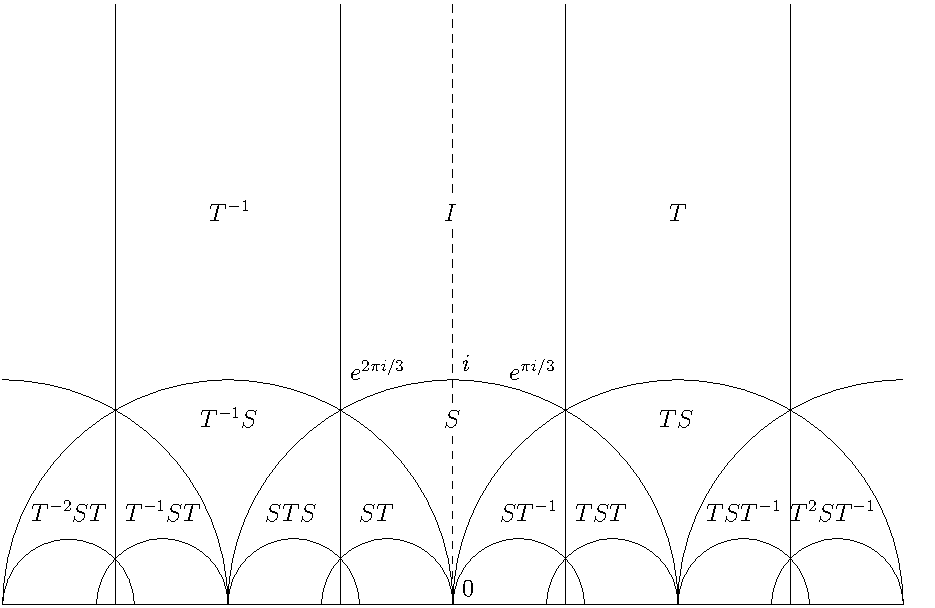
\includegraphics[scale=0.75]{fundamental.pdf}
\label{figure:tiling}
\end{figure}

If 
$\{\begin{pmatrix}a&b\\c&d\end{pmatrix}, \begin{pmatrix}-a&-b\\-c&-d\end{pmatrix}\} \in SL_2(\mathbb{R})/\{I,-I\}$ is identified with the mapping $z \mapsto \frac{az+b}{cz+d}, \mathfrak{H} \to \mathfrak{H}$, then
$SL_2(\mathbb{R})/\{I,-I\}$ is the automorphism group of the upper half plane (i.e., the group of all holomorphic bijections $\mathfrak{H} \to \mathfrak{H}$, cf. \cite[Chapter VII, \S 3]{MR1659317}).
In the next section we define modular forms, which are ``almost'' invariant under automorphisms of the upper half plane.


\section{Modular forms and cusp froms}
In this section we define modular forms. We prove that they have Fourier expansions. Then we define cusp forms, which are
an important class of modular forms, with $0$ constant term in their Fourier expansions. We then show that
modular forms and cusp forms constitute vector spaces, and prove a result about pointwise products of modular forms. 

We define the {\em factor of automorphy} $j(\gamma,z)$ by
$j(\gamma,z)=cz+d$
for $\gamma=\begin{pmatrix}a&b\\c&d\end{pmatrix} \in \Gamma$
and
$z \in \mathfrak{H}$.

A holomorphic function $f:\mathfrak{H} \to \mathbb{C}$ is said to be {\em holomorphic at infinity} if
$\lim_{\Im(z) \to \infty} f(z)$ exists.

\begin{definition}
For $k \in \mathbb{Z}$,
a {\em modular form of weight $k$}, with respect to $\Gamma=SL_2(\mathbb{Z})$, is a function $f:\mathfrak{H} \to \mathbb{C}$
that is holomorphic on $\mathfrak{H}$, holomorphic at infinity, and satisfies
\[
f(\gamma z)=j(\gamma,z)^k f(z)
\]
for all
$\gamma \in \Gamma, z \in \mathfrak{H}$.
The set of all modular forms of weight $k$ is denoted by $M_k(\Gamma)$.
\end{definition}


Fourier series will be important in studying modular forms and cusp forms, so we first introduce these.
We say that a function $f:\mathfrak{H} \to \mathbb{C}$ is $\omega$-periodic if $f(z+\omega)=f(z)$ for all $z \in \mathfrak{H}$.

\begin{lemma}
\label{lemma:fourier}
If $f:\mathfrak{H} \to \mathbb{C}$ is holomorphic and $1$-periodic, then
$f$ has an expansion
\begin{equation}
\label{eqn:fourier}
f(z)=\sum_{n=-\infty}^\infty a_n q^n, \quad q=e^{2\pi iz}, \quad a_n \in \mathbb{C},
\end{equation}
valid for all $z \in \mathfrak{H}$.
\end{lemma}
\begin{proof}
Let $A=\{z:0<|z|<1\}$ be the annulus obtained by removing the origin from the unit disc. We define $F:A \to \mathbb{C}$ by $F(q)=f(z)$ for all $q \in A$. Indeed, if $q=e^{2\pi iz_1}=e^{2\pi iz_2}$, then $2\pi iz_1=2\pi iz_2+2k\pi i$ for some integer $k$ and
$z_1=z_2+k$. Hence
$f(z_1)=f(z_2)$ by periodicity. Thus $F$ is well defined.

For all $q_0 \in A$, there exists a holomorphic branch of the logarithm, say $L_0$, defined in some neighborhood $V_0$ of $q_0$.
Then for all $q \in V_0$, $F(q)=f(\frac{L_0(q)}{2\pi i})$. 
Thus on $V_0 \cap A$, $F$ is the composition of holomorphic functions. Hence $F$ is holomorphic at $q_0 \in A$. Therefore $F$ is holomorphic on $A$.

Since $F$ is holomorphic on the annulus $A$, it has a Laurent expansion 
\begin{equation}
\label{eqn:laurentseries}
F(q)=\sum_{n=-\infty}^\infty a_n q^n, \quad a_n \in \mathbb{C},
\end{equation}
valid for all $q \in A$ \cite[Chapter V, Theorem 2.1]{MR1659317}, and
\[
f(z)=\sum_{n=-\infty}^\infty a_n q^n, 
\]
with $q=e^{2\pi iz}$, as desired.
\end{proof}

The expansion \eqref{eqn:fourier} is called the {\em Fourier expansion} or {\em $q$-expansion} of the function $f$.

Since $\gamma=\begin{pmatrix}1&1\\0&1\end{pmatrix} \in \Gamma$, for $f \in M_k(\Gamma)$, then
$f(\gamma z)=f(z+1)$ for all $z \in \mathfrak{H}$, i.e. $f$ is 1-periodic. Thus by Lemma \ref{lemma:fourier},
modular forms have Fourier expansions.
Let $f \in M_k(\Gamma)$ and let $g(q)=f(z)$, $q=e^{2\pi iz}, z \in \mathfrak{H}$.
There 
is an $\alpha \in \mathbb{C}$ such that
$\lim_{y \to \infty} f(x+iy)=\alpha$. Let $\epsilon>0$ be given. Then there is a $y_0>0$ such that for all $y>y_0$, $|f(x+iy)-\alpha|<\epsilon$. Let $\delta=e^{-2\pi y_0}$. Say $q$ is such that $|q|<\delta$. Now, $q=e^{2\pi i(x+iy)}$ for some $x,y$. Then $|q|=e^{-2\pi y}<\delta=e^{-2\pi y_0}$. As $\exp$ is an increasing function on $\mathbb{R}$, this implies $y>y_0$. Hence $|f(x+iy)-\alpha|<\epsilon$, and so $|g(q)-\alpha|<\epsilon$. Thus $\lim_{q \to 0} g(q)=\alpha$. Hence $g$ is bounded in a neighborhood of $q=0$, so
$a_n=0$ for all $n<0$ in its Laurent expansion \eqref{eqn:fourier}. This means that
$a_n=0$ for all $n<0$ in the Fourier expansion \eqref{eqn:fourier} of a modular form.  

We recall \cite[Chapter V, Theorem 2.1]{MR1659317} that for $0<s<S<1$, the Laurent series $\sum_{n=-\infty}^\infty a_n q^n$ in \eqref{eqn:laurentseries} converges absolutely for $q$ such that $s<|q|<S$. Thus in particular the Laurent series converges absolutely for $q=e^{-2\pi}$. This shows that the Fourier series \eqref{eqn:fourier} converges absolutely for $z=i$. Now, let $E=\{z:\Im(z) \geq 1\}$; it is clear that $|e^{2\pi iz}|$ has a maximum value $|e^{2\pi i^2}|=e^{-2\pi}$ on $E$. 
We define $M_n=|a_n|e^{-2n\pi}$ for $n=0,1,2,\ldots$. That the Fourier series \eqref{eqn:fourier} converges absolutely for $z=i$ means that $\sum_{n=0}^\infty M_n$ converges.
But $|a_ne^{2\pi inz}| \leq M_n$ for all $z \in E$. Therefore by the Weierstrass $M$-test, the Fourier series \eqref{eqn:fourier} converges uniformly on $E$.  
However, if a sequence $f_n$ converges uniformly on a set $E$ and $x$ is a limit point of $E$, then $\lim_{t \to x} \lim_{n \to \infty} f_n(t)=\lim_{n\to \infty} \lim_{t \to x} f_n(t)$ \cite[Theorem 7.11]{MR0385023}. Thus,
\begin{equation}
\label{eqn:constantterm}
\lim_{y \to \infty} f(z)=\lim_{y \to \infty} \sum_{n=0}^\infty a_n e^{2n\pi i(x+iy)}=\sum_{n=0}^\infty a_n \lim_{y \to \infty} e^{2n\pi ix}e^{-2n\pi y}=a_0.
\end{equation}
This tells us that constant term in the Fourier series of a modular form is the limit of the function at $i\infty$.

We will often need to consider modular forms with
$0$ constant term in their Fourier expansions.
Thus we make the following definition.

\begin{definition}
A {\em cusp form of weight $k$} is a modular form $f$ of weight $k$
whose Fourier expansion has a 0 constant term, i.e. $f \in M_k(\Gamma)$ and
\[
f(z)=\sum_{n=1}^\infty a_n q^n, \quad q=e^{2\pi iz}, \quad a_n \in \mathbb{C}.
\]
The set of all cusp forms of weight $k$ is denoted by $S_k(\Gamma)$. 
\end{definition}

From \eqref{eqn:constantterm}, a modular form $f$ is a cusp form if and only if $\lim_{\Im(z) \to \infty}f(z)=0$.

Suppose $k$ is odd and $f \in M_k(\Gamma)$. Let $\gamma=\begin{pmatrix}-1&0\\0&-1\end{pmatrix} \in \Gamma$. Then for all $z \in \mathfrak{H}$, 
\[
j(\gamma,z)^k=(0z-1)^k=-1,\, \quad f(z)=f(\gamma z)=j(\gamma,z)^k f(z)=-f(z),
\]
so $f$ is the zero function on $\mathfrak{H}$. Thus for all odd $k$, $M_k(\Gamma)$ contains only the zero function. 

In the following theorem we show that the modular forms of weight $k$ form a complex vector space, and that the cusp forms of weight $k$ are a subspace.

\begin{theorem}
For every integer,
$M_k(\Gamma)$ is a complex vector space and
$S_k(\Gamma)$ is a subspace of $M_k(\Gamma)$.
\end{theorem}
\begin{proof}
Let $f,g \in M_k(\Gamma)$ and $a \in \mathbb{C}$. Since $f$ and $g$ are holomorphic on $\mathfrak{H}$, $af+g$ is holomorphic on $\mathfrak{H}$, and since $\lim_{\Im(z) \to \infty} f(z)$ and $\lim_{\Im(z) \to \infty} g(z)$ exist, $\lim_{\Im(z) \to \infty} (af+g)(z)$ exists. Therefore $af+g$ is holomorphic at infinity. For $\gamma \in \Gamma$ and $z \in \mathfrak{H}$,
\begin{eqnarray*}
(af+g)(\gamma z)&=&af(\gamma z)+g(\gamma z)\\
&=&aj(\gamma,z)^k f(z)+j(\gamma,z)^k g(z)\\
&=&j(\gamma,z)^k(af+g)(z),
\end{eqnarray*}
hence $af+g$ satisfies the automorphy condition. Thus $af+g \in M_k(\Gamma)$. This proves that $M_k(\Gamma)$ is a complex vector space. If $f,g \in S_k(\Gamma)$, then $\lim_{\Im(z) \to \infty}(af+g)(z)=a\lim_{\Im(z) \to \infty} f(z)+\lim_{\Im(z) \to \infty} g(z)=a\cdot 0+0=0$, and thus $af+g \in S_k(\Gamma)$. Hence $S_k(\Gamma)$ is a subspace of $M_k(\Gamma)$.
\end{proof}

For modular forms $f$ and $g$, we shall define their product $fg$ by $(fg)(z)=f(z)g(z)$. The next lemma shows that
the product of a modular form of weight $k$ and a modular form of weight $l$ is a modular form of weight $k+l$. We will use
this result later in \S \ref{section:vs}.

\begin{lemma}
If $f \in M_k(\Gamma)$ and $g \in M_l(\Gamma)$, then $fg \in M_{k+l}(\Gamma)$.
\end{lemma}
\begin{proof}
It is immediate that $fg$ is holomorphic on $\mathfrak{H}$ and holomorphic at infinity. Let $\gamma \in \Gamma$ and $z \in \mathfrak{H}$. Then
\begin{eqnarray*}
(fg)(\gamma z)&=&f(\gamma z)g(\gamma z)\\
&=&j(\gamma,z)^k f(z) j(\gamma,z)^l g(z)\\
&=&j(\gamma,z)^{k+l} f(z)g(z)\\
&=&j(\gamma,z)^{k+l} (fg)(z),
\end{eqnarray*}
showing that $fg$ satisfies the automorphy condition. Therefore $fg$ is a modular form of weight $k+l$.
\end{proof}

\section{Eisenstein series}
Now we will explicitly construct a class of modular forms of all even weights $k>2$, the
Eisenstein series of weight $k$. In particular these will not be the zero function,
thus giving us nontrivial examples of modular forms. Moreover, these are not cusp forms. In fact, we will show later in this
section that for even $k>2$, any modular form of weight $k$ is a linear combination of an Eisenstein series of weight $k$
and a cusp form of weight $k$.

\begin{definition}
The {\em Eisenstein series $G_k(\tau)$ of weight $k$} 
is defined by
\[
G_k(\tau)={{\sum}'}_{c,d} \frac{1}{(c\tau+d)^k}
\]
for $\tau \in \mathfrak{H}$, where the primed summation means that summation is over
all $(c,d) \in \mathbb{Z}^2$ such that $(c,d) \neq (0,0)$.
\end{definition}

In the following theorem we prove that for all even $k \geq 4$, the Eisenstein series $G_k$ is a nonzero modular form of weight $k$. This will be our first example of a modular form (aside from the zero function). The proof follows \cite[Theorem 1, Chapter III]{MR0412107}.

\begin{theorem}
For all even integers $k \geq 4$, the Eisenstein series $G_k$ is a modular form of weight $k$.
\end{theorem}
\begin{proof}
We will use the fact \cite[Chapter V, \S 1]{MR1659317} that the series defining the Riemann zeta function
$\zeta(s)=\sum_{n=1}^\infty n^{-s}$ converges absolutely for $\Re(s)>1$.
First we show that the series $G_k(\tau)$ defines a holomorphic function $\mathfrak{H} \to \mathbb{C}$.
Let $K$ be a compact subset of $\mathfrak{H}$. Let $S^1=\{(x,y) \in \mathbb{R}^2 | x^2+y^2=1\}$ be the unit circle
in $\mathbb{R}^2$. Recall that $S^1$ is a compact subset of $\mathbb{R}^2$.
Thus the product $K \times S^1$ is a compact subset of $\mathfrak{H} \times \mathbb{R}^2$.
Clearly, $(\tau,x,y) \mapsto |x\tau+y|$ is a continuous function $K \times S^1 \to \mathbb{R}$. Hence
it attains a minimum value $\mu$.
For all $\tau \in K$ and $m_1,m_2 \in \mathbb{Z}$ with $(m_1,m_2)\neq (0,0)$,
\begin{eqnarray*}
|m_1\tau+m_2|^2&=&|\frac{m_1}{m_1^2+m_2^2}\tau+\frac{m_2}{m_1^2+m_2^2}|^2(m_1^2+m_2^2)^2\\
&\geq&\mu^2(m_1^2+m_2^2).
\end{eqnarray*}
Thus for all $\tau \in K$,
$G_k(\tau)$ is bounded above by the series
\[
\mu^{-k} {{\sum}'}_{m_1,m_2} (m_1^2+m_2^2)^{-k/2}.
\]

Now,
\[
{{\sum}'}_{m_1,m_2}(m_1^2+m_2^2)^{-k/2} = \sum_{N=1}^\infty \sum_{m_1,m_2} (m_1^2+m_2^2)^{-k/2}
\]
where the inner summation is over those $m_1,m_2 \in \mathbb{Z}$ such that
$|m_1|=N$ and $|m_2| \leq N$, or $|m_2|=N$ and $|m_1| \leq N$.
Fixing $N$, there are a most $2\cdot 2\cdot (2N+1)=8N+4$ such
pairs $(m_1,m_2) \in \mathbb{Z}^2$. Thus
\[
\sum_{N=1}^\infty \sum_{m_1,m_2} (m_1^2+m_2^2)^{-k/2} \leq \sum_{N=1}^\infty (8N+4)(N^2)^{-k/2}=\sum_{N=1}^\infty 8N^{-k+1}+4N^{-k}.
\]
We have shown that $\mu^{-k} \sum_{N=1}^\infty 8N^{-k+1}+4N^{-k}$ is an upper bound for $G_k(\tau)$.
Since $k>2$, the latter series converges, so by the 
Weierstrass $M$-test, 
$G_k(\tau)$ converges uniformly (and absolutely) on $K$.

This proves that $G_k(\tau)$ converges uniformly on compact subsets of $\mathfrak{H}$.
Therefore according to \cite[Theorem 1.1, Chapter V]{MR1659317},
$G_k$ is a holomorphic function on $\mathfrak{H}$.

We now show that $G_k$ satisfies the automorphy condition.
Let $\tau \in \mathfrak{H}$ and $\gamma=\begin{pmatrix}a&b\\c&d\end{pmatrix} \in \Gamma$. Then
\begin{eqnarray}
G_k(\gamma \tau)&=&G_k(\frac{a\tau+b}{c\tau+d})\nonumber \\
&=&{{\sum}'}_{m_1,m_2} (m_1\frac{a\tau+b}{c\tau+d}+m_2)^{-k}\nonumber \\
&=&{{\sum}'}_{m_1,m_2} (\frac{m_1a\tau+m_1b+m_2c\tau+m_2d}{c\tau+d})^{-k}\nonumber \\
&=&(c\tau+d)^k {{\sum}'}_{m_1,m_2}((m_1a+m_2c)\tau+m_1b+m_2d)^{-k}\label{eqn:eis1}.
\end{eqnarray}
Since $ad-bc=1$, $(m_1,m_2) \mapsto (m_1a+m_2c,m_1b+m_2d)$ is a bijection
$\mathbb{Z}^2 \to \mathbb{Z}^2$, by the Euclidean algorithm \cite[\S 12.3]{MR568909}. Thus, after changing variables,
\begin{equation}
\label{eqn:eis2}
{{\sum}'}_{m_1,m_2}((m_1a+m_2c)\tau+m_1b+m_2d)^{-k}={{\sum}'}_{m_1,m_2}(m_1\tau+m_2)^{-k}=G_k(\tau).
\end{equation}
Combining \eqref{eqn:eis1} with \eqref{eqn:eis2},
\[
G_k(\gamma \tau)=(c\tau+d)^kG_k(\tau)=j(\gamma,\tau)^kG_k(\tau).
\]
Finally we show that $G_k$ is holomorphic at infinity.
For $\gamma=\begin{pmatrix}1&1\\0&1\end{pmatrix} \in \Gamma$ and $\tau \in \mathfrak{H}$, we have
$G_k(\gamma \tau)=G_k(\frac{1\tau+1}{0\tau+1})=G_k(\tau+1)$. But since $G_k$ satisfies the automorphy condition,
then $G_k(\gamma \tau)=j(\gamma,z)^kG_k(\tau)=(0\tau+1)^kG_k(\tau)=G_k(\tau)$, and so $G_k(\tau+1)=G_k(\tau)$. That is,
$G_k$ is  1-period.
Since $G_k$ is holomorphic on $\mathfrak{H}$ with period 1, by Lemma \ref{lemma:fourier} it has a Fourier expansion 
\[
G_k(\tau)=\sum_{n=-\infty}^\infty a_n e^{2\pi i\tau n}, \quad \tau \in \mathfrak{H}.
\]

Now, since $k$ is even and $G_k(\tau)$ converges absolutely,
\[
G_k(\tau)=2\zeta(k)+2\sum_{m_1=1}^\infty \sum_{m_2=-\infty}^\infty (m_1\tau+m_2)^{-k}.
\]
For $m_1=1$, the inner series is $\sum_{n=-\infty}^\infty (\tau+n)^{-k}$. It
follows from the Weierstrass $M$-test that the series $\sum_{n=-\infty}^{-1} (\tau+n)^{-k}$
and $\sum_{n=0}^\infty (\tau+n)^{-k}$ converge uniformly on every compact subset of $\mathfrak{H}$ and hence define
holomorphic functions on $\mathfrak{H}$. Therefore $\sum_{n=-\infty}^\infty (\tau+n)^{-k}$ defines a holomorphic
function on $\mathfrak{H}$. Certainly $\sum_{n=-\infty}^\infty (\tau+n)^{-k}$ is 1-periodic. Thus it has a Fourier
expansion
\[
\sum_{n=-\infty}^\infty (\tau+n)^{-k}=\sum_{\nu=-\infty}^\infty \alpha_\nu e^{2\pi i\tau \nu}.
\]
Then by Laurent's formula \cite[Chapter V, Theorem 2.1]{MR1659317}, for an arbitrary $\tau_0 \in \mathfrak{H}$,
\[
\alpha_\nu=\int_{\tau_0}^{\tau_0+1} (\sum_{n=-\infty}^\infty (\tau+n)^{-k})e^{-2\pi i\nu \tau} d\tau.
\]
Since $k$ is even and $k \geq 2$, the series converges uniformly so we can interchange integration and summation
\begin{eqnarray}
\alpha_\nu&=&\sum_{n=-\infty}^\infty \int_{\tau_0}^{\tau_0+1} (\tau+n)^{-k} e^{-2\pi i\nu \tau}d\tau\nonumber \\
&=&\int_{-\infty+iy_0}^{\infty+iy_0} \tau^{-k}e^{-2\pi i\nu \tau}d\tau \label{eqn:eisII}
\end{eqnarray}
where $\Im(\tau_0)=y_0$.

Put $\tau=x+iy_0$.
Thus
\begin{eqnarray*}
|\alpha_\nu|&\leq&e^{2\pi \nu y_0} \int_{-\infty}^\infty |x+iy_0|^{-k}d\tau\\
&=&e^{2\pi \nu y_0} \int_{-\infty}^\infty (x^2+y_0^2)^{-k/2}d\tau\\
&=&e^{2\pi \nu y_0}y_0^{1-k} \int_{-\infty}^\infty (x^2+1)^{-k/2}dx.
\end{eqnarray*} 
This integral converges to some $c_k$ since $k \geq 2$.
Thus
\[
|\alpha_\nu| \leq \frac{e^{2\pi \nu y_0}}{y_0^{k-1}}c_k.
\]
Since we can choose $y_0$ to be arbitrarily large,  it follows that
\[
\alpha_\nu=0 \quad \textrm{for all $\nu \leq 0$}.
\]

For $\nu>0$,
we integrate $\tau^{-k}e^{-2\pi i\nu \tau}$ along the oriented paths in Figure \ref{figure1}, where
$y_1<0$ is arbitrary,
and apply the residue formula \cite[Theorem 1.2, Chapter VI]{MR1659317} to obtain
\begin{equation}
\label{eqn:eisI}
\int_{\textrm{I}} \tau^{-k}e^{-2\pi i\nu \tau}d\tau=\int_{\textrm{II+III+IV}} \tau^{-k}e^{-2\pi i\nu \tau}d\tau-\Res(\tau^{-k}e^{-2\pi i\nu \tau};0).
\end{equation}

\begin{figure}
\caption{Paths of integration for $\tau^{-k}e^{-2\pi i\nu \tau}$ (only singularity is pole at origin)}
\begin{center}
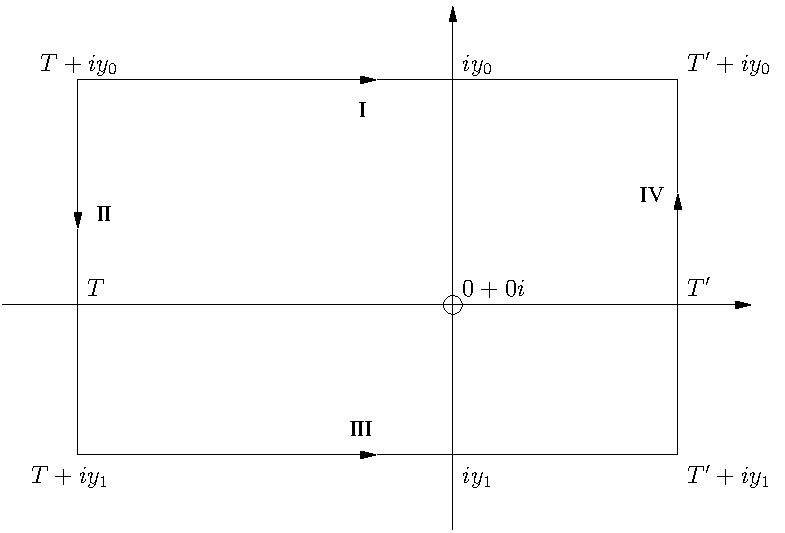
\includegraphics[scale=0.75]{fig1.pdf}
\end{center}
\label{figure1}
\end{figure}

On path II,
\begin{eqnarray*}
|\tau^{-k}e^{-2\pi i\nu \tau}|&=&|T+iy|^{-k}|e^{-2\pi i\nu(T+iy)}|\\
&=&(T^2+y^2)^{-k/2}e^{2\pi \nu y}\\
&\leq&(T^2+0^2)^{-k/2}e^{2\pi \nu y_0}\\
&=&T^{-k} e^{2\pi \nu y_0}.
\end{eqnarray*}
That is, an upper bound for $|\tau^{-k}e^{-2\pi i\nu \tau}|$ on path II is
$T^{-k} e^{2\pi \nu y_0}$.
The length of path II is $y_0-y_1$. Thus by \cite[Theorem 2.3, Chapter III]{MR1659317} we have
the estimate
\[
|\int_{\textrm{II}} \tau^{-k}e^{-2\pi i\nu \tau}d\tau| \leq T^{-k} e^{2\pi \nu y_0}(y_0-y_1).
\]
The limit of the righthand side of this inequality as $T \to -\infty$ is 0. Hence
$\lim_{T \to -\infty} \int_{\textrm{II}} \tau^{-k}e^{-2\pi i\nu \tau}d\tau=0$.

Similarly on path IV,
\begin{eqnarray*}
|\tau^{-k}e^{-2\pi i\nu \tau}|&=&|T'+iy|^{-k}|e^{-2\pi i\nu(T'+iy)}|\\
&=&(T'^2+y^2)^{-k/2}e^{2\pi \nu y}\\
&\leq&T'^{-k} e^{2\pi \nu y_0}.
\end{eqnarray*}
The length of path IV is $y_0-y_1$, so we have the estimate
\[
|\int_{\textrm{IV}} \tau^{-k}e^{-2\pi i\nu \tau}d\tau| \leq T'^{-k} e^{2\pi \nu y_0}(y_0-y_1).
\]
Hence
$\lim_{T' \to \infty} \int_{\textrm{IV}} \tau^{-k}e^{-2\pi i\nu \tau}d\tau=0$.

For path III,
\begin{eqnarray*}
|\tau^{-k}e^{-2\pi i\nu \tau}|&=&|x+iy_1|^{-k}|e^{-2\pi i\nu(x+iy_1)}|\\
&=&|x+iy_1|^{-k}e^{2\pi \nu y_1}\\
&\leq&y_1^{-k},
\end{eqnarray*}
hence
\begin{eqnarray*}
|\int_{\textrm{III}} \tau^{-k}e^{-2\pi i\nu \tau}d\tau|&\leq&|\int_T^{T'} (x^2+y_1^2)^{-k} e^{2\pi \nu y_1}dx\\
&=&e^{2\pi \nu y_1} \int_T^{T'} (x^2+y_1^2)^{-k} dx.
\end{eqnarray*}
However, $\int_{-\infty}^\infty \frac{1}{(x^2+y_1^2)^k} dx=\frac{\pi}{2^{k-1}} \frac{1\cdot 3\cdots (2k-3)}{1\cdot 2\cdots (k-1)} \frac{1}{y^{2k-1}}$ \cite[Chapter XV, \S 2, K7]{MR1659317}.
Thus the absolute value of the above integral is bounded above 
by $e^{2\pi \nu y_1}\frac{\pi}{2^{k-1}} \frac{1\cdot 3\cdots (2k-3)}{1\cdot 2\cdots (k-1)} \frac{1}{y^{2k-1}}$.

Since $y_1<0$ is arbitrary, it must be that
\[
\lim_{T \to -\infty} \lim_{T' \to \infty} \int_{\textrm{III}} \tau^{-k}e^{-2\pi i\nu \tau}d\tau=0.
\]

Therefore \eqref{eqn:eisI} reduces to
\[
\int_{-\infty+iy_0}^{\infty+iy_0} \tau^{-k}e^{-2\pi i\nu \tau}d\tau=-\Res(\tau^{-k}e^{-2\pi i\nu \tau};0).
\]
Now, the Laurent series of $\tau^{-k}e^{-2\pi i\nu \tau}$ is
\begin{eqnarray*}
\tau^{-k}e^{-2\pi i\nu \tau}&=&\tau^{-k} \sum_{l=0}^\infty \frac{(-2\pi i\nu)^l \tau^l}{l!}\\
&=&\sum_{l=0}^\infty \frac{(-2\pi i\nu)^l \tau^{l-k}}{l!}.
\end{eqnarray*}
Thus $\Res(\tau^{-k}e^{-2\pi i\nu \tau};0)=\frac{(-2\pi i\nu)^{k-1}}{(k-1)!}$.
Hence
\[
\int_{-\infty+iy_0}^{\infty+iy_0} \tau^{-k}e^{-2\pi i\nu \tau}d\tau=(-2\pi i)^k \frac{\nu^{k-1}}{(k-1)!}.
\]
By \eqref{eqn:eisII} we have
\[
\alpha_\nu=(-2\pi i)^k \frac{\nu^{k-1}}{(k-1)!},
\]
giving us the Fourier series when $m_1=1$.

Then for $m_1>1$,
\[
\sum_{n=-\infty}^\infty (m_1\tau+n)^{-k}=\sum_{\nu=1}^\infty \alpha_\nu e^{2\pi i\nu m_1\tau},
\]
hence
\begin{eqnarray}
\nonumber
G_k(z)&=&2\zeta(k)+2\sum_{m_1=1}^\infty \frac{(2\pi i)^k}{(k-1)!} \sum_{\nu=1}^\infty \nu^{k-1} e^{2\pi im_1 \nu z}\\
&=&2\zeta(k)+\frac{2(2\pi i)^k}{(k-1)!} \sum_{n=1}^\infty \sigma_{k-1}(n)e^{2\pi i nz}\label{eqn:Gfourier},
\end{eqnarray}
where $\sigma_r(n)$ is the sum of the $r$th powers of the positive divisors of $n$, e.g. $\sigma_r(6)=1^r+2^r+3^r+6^r$.

Therefore $\lim_{\Im(z) \to \infty} G_k(z)= 2\zeta(k)$. Hence
$G_k$ is holomorphic at infinity, and the constant term in the Fourier expansion of $G_k$ is $2\zeta(k)$. Since $\zeta(k)=\sum_{n=1}^\infty n^{-k} \neq 0$, $G_k$ is not the zero function.
\end{proof}

For even $k \geq 4$, in the following theorem we show that $M_k(\Gamma)$ decomposes into an internal direct sum of the cusp forms $S_k(\Gamma)$ and multiples of the Eisenstein series $G_k$. 

\begin{theorem}
For all even $k \geq 4$,
\[
M_k(\Gamma)=S_k(\Gamma) \oplus G_k\mathbb{C}.
\]
\end{theorem}
\begin{proof}
For $f \in M_k(\Gamma)$, $f$ has a Fourier expansion
\[
f(z)=\sum_{n=0}^\infty a_n e^{2\pi iz}, \quad a_n \in \mathbb{C}.
\] 
Let $h=f-\frac{a_0}{2\zeta(k)}G_k$. Then $h \in S_k(\Gamma)$, and $f=h+\frac{a_0}{2\zeta(k)}G_k$ where $\frac{a_0}{2\zeta(k)}G_k \in G_k\mathbb{C}$. Furthermore, the only multiple of $G_k$ with zero constant term in its Fourier expansion is the zero function. Hence the intersection of $S_k(\Gamma)$ and $G_k\mathbb{C}$ is the zero subspace of $M_k(\Gamma)$. Thus $M_k(\Gamma)=S_k(\Gamma) \oplus G_k\mathbb{C}$. 
\end{proof}

\section{The Dedekind eta function}
We would like to give an explicit example of a nonzero cusp form. We will construct this using the following function.

\begin{definition}
The {\em Dedekind eta function} $\eta:\mathfrak{H} \to \mathbb{C}$ is defined by 
\begin{equation}
\label{eqn:eta1}
\eta(z)=q^{1/24} \prod_{n=1}^\infty (1-q^n)
\end{equation}
for $q=e^{2\pi iz}$.
\end{definition}

We will now show that the Dedekind eta function is holomorphic on $\mathfrak{H}$ and has no zeros in $\mathfrak{H}$.
This will be done by showing that the infinite product defining $\eta$ converges uniformly on all
compact subsets of $\mathfrak{H}$. We will prove the uniform convergence of this infinite product
by results about the uniform convergence of series.

Let $a_n$ be a sequence of complex numbers such that the series $\sum_{n=1}^\infty \log(1+a_n)$ converges. Here $\log(1+z)=-\sum_{n=1}^\infty \frac{z^n}{n}$ for $|z-1|<1$ (the open unit disc with center $1+0i$).
For all $N$, $\exp(\sum_{n=1}^N \log(1+a_n))=\prod_{n=1}^N (1+a_n)$.
Since the exponential function is continuous, we have $\prod_{n=1}^\infty (1+a_n)=\exp(\sum_{n=1}^\infty \log(1+a_n)) \neq 0$.

Let $K$ be a compact subset of $\mathfrak{H}$.
Let $z_0 \in K$ such that $|e^{2\pi iz_0}|$ is maximum, and put $q_0=e^{2\pi iz_0}$.
Since $|q_0|<1$, there is some $m$ such that for all $n \geq m$, $|q_0^n| < \frac{1}{2}$.
Now, let $z \in K$, and put $q=e^{2\pi iz}$.
For all $n \geq m$,
\begin{eqnarray*}
|\log(1-q^n)|&\leq&|q^n|+\frac{|q^n|^2}{2}+\ldots\\
&\leq&|q_0^n|+\frac{|q_0^n|^2}{2}+\ldots\\
&\leq&|q_0^n|+|q_0^n|^2+\ldots\\
&=&|q_0^n| \frac{1}{1-|q_0^n|}\\
&<&|q_0^n| \frac{1}{1-\frac{1}{2}}\\
&=&2|q_0^n|.
\end{eqnarray*}
But the series $\sum_{n=m}^\infty |q_0|^n$ converges (since $|q_0|<1$). Hence by the Weierstrass $M$-test, $\sum_{n=1}^\infty \log(1-e^{2\pi inz})$ converges uniformly on $K$.

Let $h_m$ be a sequence of continuous functions that converge uniformly on $K$ to a (continuous) function $h$. Then
there exists an $N$ such that for all $m \geq N$, $|h_m(z)-h(z)|<1$ for all $z \in K$.
Since $h$ is continuous, $h(K)$ is compact, hence it is contained in a closed disc, of radius $r$. Let $D$ be the closed concentric disc with radius $r+1$. Then $h_m(K) \subseteq D$ for all $m \geq N$. Now let $\epsilon>0$ be given. Since $\exp$ is continuous on the compact set $D$, it is uniformly continuous on $D$ \cite[Theorem 4.19]{MR0385023}. Hence there exists a $\delta>0$ such that if $w_1,w_2 \in D$ and $|w_1-w_2|<\delta$, then $|\exp(w_1)-\exp(w_2)|<\epsilon$.
But since $h_m \to h$ uniformly on $K$, there exists an $M \geq N$ such that for all $m \geq M$, $|h_m(z)-h(z)|<\delta$ for all $z \in K$. So $|\exp(h_m(z))-\exp(h(z))|<\epsilon$ for all $m \geq M, z \in K$. Thus ${\exp}\circ h_m$ converges uniformly on $K$ to ${\exp}\circ h$.
Setting $h_m=\sum_{n=1}^m \log(1-e^{2\pi inz})$, we find that the infinite product $\prod_{n=1}^\infty (1-e^{2\pi inz})$ converges uniformly on $K$.

Since the infinite product $\prod_{n=1}^\infty (1-e^{2\pi inz})$ converges uniformly on all compact subsets of $\mathfrak{H}$, 
$\eta(z)=e^{\pi iz/12}\prod_{n=1}^\infty (1-e^{2\pi inz})$ is a holomorphic function $\mathfrak{H} \to \mathbb{C}$ \cite[Chapter V, Theorem 1.1]{MR1659317}.
As $\eta(z)=e^{\pi iz/12}\exp(\sum_{n=1}^\infty \log(1-e^{2\pi inz}))$ for all $z \in \mathfrak{H}$, $\eta(z) \neq 0$ for all $z \in \mathfrak{H}$.

The following theorem shows how $\eta$ transforms under $B=\begin{pmatrix}0&-1\\1&0\end{pmatrix}$, one of the two generators of the modular group $\Gamma$, by Theorem \ref{theorem:generate}. After this theorem, we can then show how $\eta$ transforms under the whole modular group $\Gamma$.
Our proof of the following theorem follows \cite[Theorem 2, Chapter VIII]{MR808396}.

\begin{theorem}
\label{thm:eta}
For all $z \in \mathfrak{H}$,
\[
\eta(\frac{-1}{z})=\sqrt{\frac{z}{i}} \cdot \eta(z),
\]
where $\sqrt{\,}$ is the principal branch of the square root, holomorphic on the plane with the ray $\{z \in \mathbb{C}:\Im(z)=0, \Re(z) \leq 0\}$ removed.
\end{theorem}
\begin{proof}
$\eta(\frac{-1}{z})$ and $\sqrt{\frac{z}{i}} \cdot \eta(z)$ are holomorphic functions of $z$ on $\mathfrak{H}$. If they are equal on a set with an accumulation point in $\mathfrak{H}$ then they are equal on all of $\mathfrak{H}$ by the identity theorem for holomorphic functions \cite[Chapter III, Theorem 1.2]{MR1659317}.
It therefore suffices to prove the theorem for purely imaginary $z=iy, y>0$. Suppose now that $z=iy,y>0$. 

Since $\eta(z) \neq 0$ for $y>0$, we can take logarithms in \eqref{eqn:eta1}, and use the series expansion
\[
\log(1-e^{2\pi imz})=-\sum_{k=1}^\infty \frac{1}{k}e^{2\pi ikmz}, \quad \Im(z)>0, \quad m=1,2,\ldots
\]
to obtain
\begin{equation}
\label{eqn:eta2}
\log \eta(z)=\frac{\pi iz}{12}+\sum_{m=1}^\infty \log(1-e^{2\pi imz})=\frac{\pi iz}{12}-\sum_{m=1}^\infty \sum_{k=1}^\infty \frac{1}{k} e^{2\pi ikmz}.
\end{equation}
The double series converges absolutely, because $|e^{2\pi ikmz}|=e^{-2\pi kmy}, y>0$.

Since $\Im(z)>0$, we have $\Im(-\frac{1}{z})>0$. We can therefore replace $z$ with $-\frac{1}{z}$ in \eqref{eqn:eta2} to obtain
\begin{equation}
\label{eqn:eta3}
\log \eta(-\frac{1}{z})=-\frac{\pi i}{12z}-\sum_{m=1}^\infty \sum_{k=1}^\infty \frac{1}{k} e^{-2\pi ikm/z}.
\end{equation}
Since
\[
\sum_{m=1}^\infty e^{2\pi ikmz}=\frac{e^{2\pi ikz}}{1-e^{2\pi ikz}} \quad \textrm{and} \quad
\sum_{m=1}^\infty e^{-2\pi ikm/z}=\frac{e^{-2\pi ik/z}}{1-e^{-2\pi ik/z}},
\]
to prove to the theorem it suffices, by \eqref{eqn:eta2} and \eqref{eqn:eta3}, to prove
\begin{equation}
\label{eqn:eta4}
-\frac{\pi iz}{12}-\frac{\pi i}{12z}+\sum_{k=1}^\infty \frac{1}{k}(\frac{e^{2\pi ikz}}{1-e^{2\pi ikz}}-\frac{e^{-2\pi ik/z}}{1-e^{-2\pi ik/z}})=\frac{1}{2}\log \frac{z}{i}.
\end{equation}

Now, the $n$th partial sum of the infinite series in \eqref{eqn:eta4} can be written as
\begin{equation}
\label{eqn:cot}
\begin{split}
&\quad \sum_{k=1}^n \frac{1}{2k}(\frac{2e^{2\pi ikz}}{1-e^{2\pi ikz}}+1-\frac{2e^{-2\pi ik/z}}{1-e^{-2\pi ik/z}}-1)\\
&=\sum_{k=1}^n \frac{i}{2k}(-i\frac{1+e^{2\pi ikz}}{1-e^{2\pi ikz}}+i\frac{1+e^{-2\pi ik/z}}{1-e^{-2\pi ik/z}})\\
&=\sum_{k=1}^n \frac{i}{2k}(\cot \pi kz+\cot \frac{\pi k}{z})\\
&=\sum_{\stackrel{k=-n}{k \neq 0}}^n \frac{i}{4k}(\cot \pi kz+\cot \frac{\pi k}{z}),
\end{split}
\end{equation}
where $\cot s=i\frac{e^{2is}+1}{e^{2is}-1}=\frac{\cos s}{\sin s}$ is the cotangent function.

To prove the theorem, by \eqref{eqn:cot} it suffices to prove that
\begin{equation}
\label{eqn:eta5}
-\frac{\pi i}{12}(z+\frac{1}{z})+\sum_{\stackrel{k=-n}{k \neq 0}}^n \frac{i}{4k}(\cot \pi kz+\cot \frac{\pi k}{z})\to \frac{1}{2}\log \frac{z}{i}, \quad \textrm{as $n \to +\infty$}.
\end{equation}
This will be done by applying the residue theorem to a certain path integral, of a suitably chosen function.

Let
\begin{equation}
\varphi(s)=\cot s \cdot \cot \frac{s}{z}, \quad \nu=\pi(n+\frac{1}{2}),
\end{equation}
Since $\sin(s)=\frac{e^{is}-e^{-is}}{2i}$ has a simple zero at $s=n\pi$ and no other zeros,
and $\cos(s)=\frac{e^{is}+e^{-is}}{2}$ has a simple zero at $n\pi+\pi/2$ and no other zeros,
$n \in \mathbb{Z}$, the function $\cot(s)$ has a simple zero at $s=n\pi i+\pi/2$ and a simple pole at $s=n\pi$, $n \in \mathbb{Z}$,
and no other zeros or poles.
Therefore $\frac{\varphi(\nu s)}{s}$ is meromorphic, with simple poles at $s=\frac{\pi k}{\nu}$ and $s=\frac{\pi k}{\nu}z$, where $k$ is any nonzero integer, and a triple pole at $s=0$, and has no other poles.

The Laurent expansion of $\frac{\varphi(\nu s)}{s}$ about $s=0$ is found by noting that
\begin{eqnarray*}
\cot s&=&\frac{\cos s}{\sin s}\\
&=&\frac{1-\frac{s^2}{2}+\ldots}{s(1-\frac{s^2}{6}+\ldots)}\\
&=&\frac{1}{s}(1-\frac{s^2}{2}+\ldots)(1+\frac{s^2}{6}+\ldots)\\
&=&\frac{1}{s}-\frac{s}{3}+\ldots,
\end{eqnarray*}
and so
\[
\frac{\varphi(\nu s)}{s}=\frac{1}{s}(\frac{1}{\nu s}-\frac{\nu s}{3}+\ldots)(\frac{z}{\nu s}-\frac{\nu s}{3z}+\ldots).
\]
Furthermore, $\cot s$ has period $\pi$, because
\[
\cot(s+\pi)=i\frac{e^{2i(s+\pi)}+1}{e^{2i(s+\pi)}-1}=i\frac{e^{2is}+1}{e^{2is}-1}=\cot s.
\]
Thus the Laurent series of $\cot(\nu s)$ about $s=\frac{\pi k}{\nu}$ is
\[
\frac{1}{\nu s-\pi k}-\frac{\nu s-\pi k}{3}+\ldots=\frac{1}{\nu(s-\frac{\pi k}{\nu})}-\frac{\nu(s-\frac{\pi k}{\nu})}{3}+\ldots,
\]
and the Laurent series of $\cot(\frac{\nu s}{z})$ about $s=\frac{\pi k}{\nu}z$ is
\[
\frac{1}{\frac{\nu s}{z}-\pi k}-\frac{\frac{\nu s}{z}-\pi k}{3}+\ldots =\frac{z}{\nu(s-\frac{\pi k}{\nu}z)}-\frac{\nu(s-\frac{\pi k}{\nu}z)}{3z}+\ldots.
\]
The residues of $\frac{\varphi(\nu s)}{s}$ at $s=0$, $s=\frac{\pi k}{\nu}$, and $s=\frac{\pi k}{\nu}z$ are respectively
\[
-\frac{1}{3}(z+\frac{1}{z}),\quad \frac{\nu}{\pi k}\Res(\cot(\nu s);\frac{\pi k}{z})\cot \frac{\pi k}{z},\quad \frac{\nu}{\pi k z}\cot(\pi k z)\Res(\cot \frac{\nu s}{z};\frac{\pi k}{\nu}z),
\]
i.e.
\[
-\frac{1}{3}(z+\frac{1}{z}),\quad \frac{1}{\pi k}\cot \frac{\pi k}{z}, \quad \frac{1}{\pi k}\cot \pi kz.
\]

\begin{figure}
\caption{Paths of integration of $\frac{\varphi(\nu s)}{s}$, $\nu=\pi(n+\frac{1}{2})$}
\begin{center}
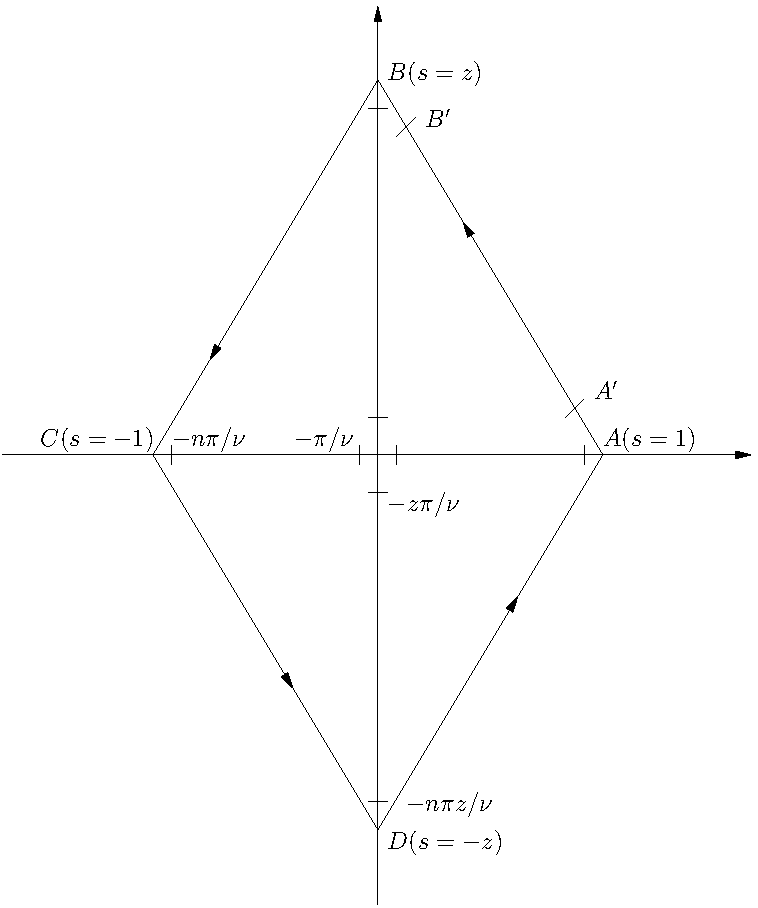
\includegraphics[scale=0.75]{eta1.pdf}
\end{center}
\label{figure:etaP}
\end{figure}

Let $P$ denote the parallelogram with vertices at $A (s=1)$, $B(s=z=iy)$, $C(s=1)$ and $D(s=-z=-iy)$ oriented counterclockwise, 
shown in Figure \ref{figure:etaP}. Then since $\nu=\pi(n+\frac{1}{2})$, the residue theorem implies that
\[
\frac{1}{2\pi i}\int_P \frac{\varphi(\nu s)}{s} ds=-\frac{1}{3}(z+\frac{1}{z})+\sum_{\stackrel{k=-n}{k \neq 0}}^n \frac{1}{\pi k}(\cot \pi kz+\cot \frac{\pi k}{z}).
\]
Here the initial term is the residue of $\frac{\varphi(\nu s)}{s}$ at the triple pole $s=0$, and the summation is over the residues of $\frac{\varphi(\nu s)}{s}$ at the simple poles $s=\frac{\pi k}{\nu}$ and $s=\frac{\pi k}{\nu}z$ respectively; the function $\frac{\varphi(\nu s)}{s}$ has no other poles inside $P$.
Thus,
\[
\int_P \frac{\varphi(\nu s)}{8s} ds=-\frac{\pi i}{12}(z+\frac{1}{z}) +\sum_{\stackrel{k=-n}{k \neq 0}}^n \frac{i}{4 k}(\cot \pi kz+\cot \frac{\pi k}{z}).
\]
To prove \eqref{eqn:eta5} it therefore suffices to prove that
\begin{equation}
\label{eqn:etaintegral1}
\lim_{n \to \infty} \int_P \frac{\varphi(\nu s)}{8s}ds=\frac{1}{2}\log \frac{z}{i}, \quad \nu=\pi(n+\frac{1}{2}).
\end{equation}


Because $\cot{s}$ has period $\pi$, and $|\cot{s}|<M_1$ for $s\in P$ with $-\frac{\pi}{2} \leq \Re(s) \leq \frac{\pi}{2}$, $|s| \geq \delta_0>0$ (since the only pole of $\cot{s}$ with real part between $-\pi/2$ and $\pi/2$ is $0$), it follows that
\begin{equation}
\label{eqn:inequality}
|\frac{\varphi(\nu s)}{s}|<M, \quad s \in P, \quad \nu=\pi(n+\frac{1}{2}), n=1,2,\ldots.
\end{equation}
Here $M$ is independent of $s$ and $\nu$.
As well, since
\[
\cot s=i\frac{e^{2\pi is}+1}{e^{2\pi is}-1},
\]
we have
\begin{equation}
\label{eqn:limits}
\cot s \to \begin{cases}-i,&\textrm{as $\Im(s) \to +\infty$},\\
+i,&\textrm{as $\Im(s) \to -\infty$}.\end{cases}
\end{equation}

Let $K$ be a compact subset of the upper half plane $\mathfrak{H}$, and let $\epsilon>0$. As $\nu \to \infty$, $\Im(\nu s) \to \infty$ for $s \in K$. Thus by \eqref{eqn:limits}, $\cot \nu s \to -i$ as $\nu \to \infty$ uniformly for $s \in K$ (since as $K$ is compact, there is an $s \in K$ such that $\Im(s)$ is minimum). Similarly,
$\cot \nu s \to +i$ as $\nu \to +\infty$ uniformly in every compact set in the lower half plane $\Im(s)<0$,
$\cot \frac{\nu s}{z} \to -i$ as $\nu \to +\infty$ uniformly in every compact set in the left half plane $\Re(s)<0$, and $\cot \frac{\nu s}{z}\to +i$ as $\nu \to +\infty$ uniformly in every compact set in the right half plane $\Re(s)>0$.


To prove \eqref{eqn:etaintegral1}, we shall show that
\begin{equation}
\label{eqn:etaintegrals2}
\lim_{n \to \infty} \int_P \frac{\varphi(\nu s)}{s}ds=(\int_1^z  - \int_z^{-1}  + \int_{-1}^{-z}  - \int_{-z}^1) \frac{ds}{s},
\end{equation}
where the integrals on the right hand side are along the respective paths $AB$, $BC$, $CD$, $DA$ of the parallelogram $P$. We will then show that the sum of the integrals on the right hand side is equal to $4\log \frac{z}{i}$, which would prove \eqref{eqn:etaintegral1}.

We first split the integral along the path $AB$ into three parts, from $A$ to $A'$, $A'$ to $B'$, and $B'$ to $B$, such that the distances $|AA'|$ and $|B'B|$ are equal to $\delta>0$, to be chosen sufficiently small. 
From above, $\varphi(\nu s) \to (+i)(-i)=1$ uniformly as $\nu \to \infty$, for $s$ in the compact set $A'B'$. Therefore,
for any $\epsilon'>0$ there exists a $\nu_0$ such that for all $\nu \geq \nu_0$, $|\varphi(\nu s)-1|<\epsilon'$ for $s \in A'B'$. But $|s|$ has a minimum $\delta_1>0$ on $A'B'$, so $|\frac{\varphi(\nu s)-1}{s}|<\frac{\epsilon'}{\delta_1}$ for $s \in A'B'$. 
By \eqref{eqn:inequality}, $|\frac{\varphi(\nu s)-1}{s}|<M+\frac{1}{\delta_1}$ for all $s \in AA',B'B$. Hence,
given $\epsilon>0$, there exist a $\delta>0$ and a $\nu_0$ such that for all $\nu \geq \nu_0$, we have
\begin{eqnarray*}
|\int_A^B \frac{\varphi(\nu s)-1}{s}ds|&\leq&|\int_{A'}^{B'} \frac{\varphi(\nu s)-1}{s} ds|+|\int_A^{A'}|+|\int_{B'}^B|\\
&<&|AB|\frac{\epsilon'}{\delta_0}+\delta(M+\frac{1}{\delta_1})+\delta(M+\frac{1}{\delta_1})\\
&<&\epsilon.
\end{eqnarray*}
We have just shown that
\begin{equation}
\lim_{n \to \infty} \int_A^B \frac{\varphi(\nu s)}{s}ds=\int_A^B \frac{ds}{s}=\int_1^z \frac{ds}{s}.
\end{equation}
Similar results hold for the other three edges of $P$. Thus \eqref{eqn:etaintegrals2} follows, and
\[
\lim_{n \to \infty} \int_P \frac{\varphi(\nu s)}{s}ds=2(\int_1^z \frac{ds}{s}+\int_{-1}^z \frac{ds}{s}).
\]

\begin{figure}
\caption{Simple curve $L$ joining $A$ and $C$}
\begin{center}
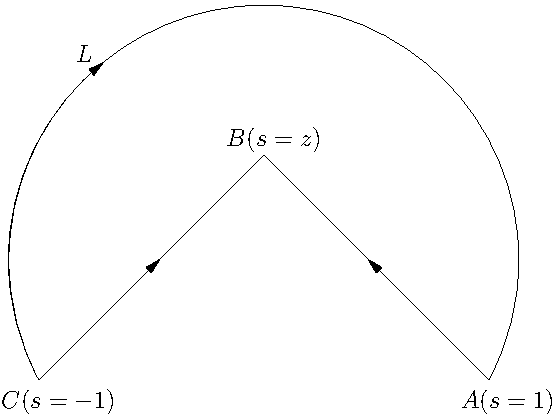
\includegraphics[scale=0.75]{arc.pdf}
\end{center}
\label{figure:circle}
\end{figure}

Let $L$ be a simple curve in the upper half plane joining $A$ and $C$ and not passing through $CB$ or $AB$, as in Figure \ref{figure:circle}.
Since $L$ is homotopic to the arc of the unit circle from $-1$ to $1$, which is parameterized by
$s=e^{it}, \pi \leq t \leq 0$, by \cite[Chapter III, Theorem 5.1]{MR1659317} we have
\[
\int_L \frac{ds}{s}=\int_{\pi}^0 \frac{d(e^{it})}{e^{it}}=\int_{\pi}^0 i dt=-\pi i.
\]
As $0$ is not in the region contained by $L$ and the line segments $CB,AB$,
by the residue theorem we have
\begin{eqnarray*}
\lim_{n \to \infty} \int_P \frac{\varphi(\nu s)}{s}ds&=&4\int_1^z \frac{ds}{s}+2\int_L \frac{ds}{s}\\
&=&4\log z -2 \cdot 2 \frac{\pi i}{2}\\
&=&4\log z-4\log i\\
&=&4\log \frac{z}{i}.
\end{eqnarray*}
This proves \eqref{eqn:etaintegral1}, and thus the theorem.
\end{proof}

The proof of the analog of the automorphy condition for $\eta$ follows \cite[Chapter VIII, Theorem 3]{MR808396}.

\begin{theorem}
\label{thm:etatransform}
Suppose $a,d,b,c$ are integers such that $ad-bc=1$. Then for all $z \in \mathfrak{H}$,
\begin{equation}
\label{eqn:functionalsqrt}
\eta(\frac{az+b}{cz+d})=\omega \sqrt{cz+d} \cdot \eta(z)
\end{equation}
where $\omega \in \mathbb{C}$ is a $24$th root of unity that depends on $a,b,c,d$, but not on $z$.
\end{theorem}
\begin{proof}
First we note that
for all $z \in \mathfrak{H}$,
\begin{equation}
\label{eqn:addition}
\eta(z \pm 1)=e^{\frac{2\pi (z \pm 1)}{24}} \prod_{n=1}^\infty (1-e^{2n\pi iz(z \pm 1)})=e^{\pm \pi i/12}\eta(z).
\end{equation}

Let $A=\begin{pmatrix}1&1\\0&1\end{pmatrix}, B=\begin{pmatrix}0&-1\\-1&0\end{pmatrix}$, and let $M=\begin{pmatrix}a&b\\c&d\end{pmatrix} \in \Gamma$. If $M=A^{\pm 1}$ or $B=B^{-1}$ then
\begin{equation}
\label{eqn:functional}
\eta(Mz)^{24}=(cz+d)^{12}\eta(z)^{24}
\end{equation}
holds because of \eqref{eqn:addition} and Theorem \ref{thm:eta} respectively. Now suppose \eqref{eqn:functional} holds
for some fixed $M=\begin{pmatrix}a&b\\c&d\end{pmatrix} \in \Gamma$. Then
\[
MA^{\pm 1}=\begin{pmatrix}a&b\\c&d\end{pmatrix}\begin{pmatrix}1&\pm 1\\0&1\end{pmatrix}=\begin{pmatrix}a&\pm a+b\\c&\pm c+d\end{pmatrix}
\]
and
\[
MB=\begin{pmatrix}a&b\\c&d\end{pmatrix}\begin{pmatrix}0&-1\\-1&0\end{pmatrix}=\begin{pmatrix}-b&-a\\-d&-c\end{pmatrix}.
\]
Hence
\[
\eta(MA^{\pm 1}z)=(c(z \pm 1)+d)^{12} \eta(z \pm 1)^{24}=(cz \pm c+d)^{12} \eta(z)
\]
by \eqref{eqn:addition}. Therefore so \eqref{eqn:functional} holds for $MA^{\pm 1}$. Furthermore
\[
\eta(MBz)^{24}=(c(\frac{-1}{z})+d)^{12} \eta(\frac{-1}{z})^{24}=(\frac{-c+dz}{z})^{12} z^{12} \eta(z)^{24}=(dz-c)^{12} \eta(z)^{24}
\]
by Theorem \ref{thm:eta}. Therefore \eqref{eqn:functional} holds for $MB=MB^{-1}$. Since $\Gamma$ is generated by $A$ and $B$, by Theorem \ref{theorem:generate}, therefore \eqref{eqn:functional} holds for all $M=\begin{pmatrix}a&b\\c&d\end{pmatrix} \in \Gamma$.

For $M=\begin{pmatrix}a&b\\c&d\end{pmatrix} \in \Gamma$,
taking the 24th roots of both sides of \eqref{eqn:functional} gives
$\eta(Mz)=\omega(z)\sqrt{cz+d}\cdot \eta(z)$ for some function $\gamma$ that takes values in the 24th roots of unity. But $\eta(Mz)$ and $\sqrt{cz+d}\cdot \eta(z)$ are continuous functions of $z$ on $\mathfrak{H}$, and $\sqrt{cz+d}\cdot \eta(z) \neq 0$ for all $z \in \mathfrak{H}$, so $\omega(z)$ is a continuous function on $\mathfrak{H}$. Since $\omega(z)$ is a continuous function from the connected set $\mathfrak{H}$ to the discrete set of $24$th roots of unity, it must be a constant $24$th root of unity $\omega$, which completes the proof.
\end{proof}

Now we can explicitly construct a cusp form. By taking the 24th powers of each side of
\eqref{eqn:functionalsqrt} we find that $\eta^{24}$ satisfies the automorphy condition $\eta(\gamma z)^{24}=j(\gamma,z)^{12}\eta(z)$
for all $\gamma \in \Gamma$ and $z \in \mathfrak{H}$. This leads us to define the following function. 

\begin{definition}
The {\em modular discriminant} $\Delta(z)$ is defined
by
\[
\Delta(z)=\eta(z)^{24}
\]
for $z \in \mathfrak{H}$.
\end{definition}

\begin{corollary}
The modular discriminant
$\Delta$ is a cusp form of weight 12.
\end{corollary}
\begin{proof}
That $\Delta$ is a holomorphic function $\mathfrak{H} \to \mathbb{C}$ and that $\Delta$ is holomorphic at infinity
follows immediately from $\Delta=\eta^{24}$.


Suppose $a,b,c,d \in \mathbb{Z}$ such that $ad-bc=1$. Then for $\gamma \in \Gamma, z \in \mathfrak{H}$, Theorem \ref{thm:etatransform} tells us that
\begin{eqnarray*}
\Delta(\gamma z)&=&\eta(\gamma z)^{24}\\
&=&(\sqrt{j(\gamma,z)}\cdot \eta(z))^{24}\\
&=&j(\gamma,z)^{12}\Delta(z).
\end{eqnarray*}
This shows that $\Delta$ satisfies the automorphy condition. Therefore $\Delta$ is a modular form of weight 12.

Moreover,
\[
\lim_{\Im(z) \to \infty}\Delta(z)=\lim_{\Im(z) \to \infty} \eta(z)^{24}=(\lim_{\Im(z) \to \infty}\eta(z))^{24}=0,
\]
showing that $\Delta$ is a cusp form of weight 12.
\end{proof}

Since $\Delta$ is a cusp form, it has a Fourier expansion $\Delta(z)=\sum_{n=1}^\infty a_n q^n$, $q=e^{2\pi iz}$. The {\em Ramanujan tau function} is defined by $\tau(n)=a_n$ for all $n$, that is, the Ramanujan tau function is defined by the 
Fourier coefficients of the modular discriminant.


We give the following estimates for the magnitude of the Fourier coefficients of cusp forms. The following estimates
will be employed in defining a certain inner product on $S_k(\Gamma)$ in \S \ref{section:vs}.
Moreover, since
the Fourier coefficients of cusp forms are related to number theoretic functions, estimates on their magnitude 
give us number theoretic information.
The proof of the following theorem follows \cite[Chapter VII, Theorem 5]{MR0344216}. 

\begin{theorem}
If $f \in S_k(\Gamma)$ with Fourier expansion
\[
f(z)=\sum_{n=1}^\infty a_n q^n, \quad q=e^{2\pi iz},
\]
then $a_n=O(n^{k/2})$ for all $n \geq 1$.
\end{theorem}
\begin{proof}
Indeed the series $\sum_{n=1}^\infty a_n q^{n-1}$ defines a holomorphic function in a closed disc $D$ about $q=0$ of radius $r$ for any $0<r<1$. Let such an $r$ be fixed. Then $\sum_{n=1}^\infty a_n q^{n-1}$ has a maximum value in the compact
set $D$.
Hence for $z=x+iy$, as $y \to \infty$,
\[
|f(z)|=O(q)=O(e^{-2\pi y}), \quad q=e^{2\pi i(x+iy)} \in D,
\] 
since for all sufficiently large $y$, $e^{2\pi i(x+iy)} \in D$.
Let $\varphi(z)=|f(z)|y^{k/2}$ for $z \in \mathfrak{H}, y=\Im(z)$. Then for all $g=\begin{pmatrix}a&b\\c&d\end{pmatrix} \in \Gamma$, $\Im(gz)=\frac{\Im(z)}{|cz+d|^2}$. Hence
\begin{eqnarray*}
\varphi(gz)&=&|f(gz)| (\frac{y}{|cz+d|^2})^{k/2}\\
&=&|(cz+d)^k f(z)| \frac{y^{k/2}}{|cz+d|^k}\\
&=&|cz+d|^k |f(z)| \frac{y^{k/2}}{|cz+d|^k}\\
&=&\varphi(z),
\end{eqnarray*}
so $\varphi$ is invariant under $\Gamma$. Since $f$ is a cusp form, $\varphi(z) \to 0$ as $y \to \infty$.
Since $\varphi$ is continuous on $\overline{F}$, the closure of the fundamental domain $F$, it is bounded on the compact set obtained by removing all
$z \in \overline{F}$ with $\Im(z)>y_0$ some $y_0>0$. Therefore for some $M>0$, $|\varphi(z)| \leq M$ for all $z \in \overline{F}$.
The invariance of $\varphi$ under $\Gamma$ implies that $|\varphi(z)|\leq M$ for all $z \in \mathfrak{H}$.
Hence 
\begin{equation}
\label{eqn:bounded}
|f(z)| \leq My^{-k/2}, \quad z \in \mathfrak{H}, y=\Im(z).
\end{equation}

Let $y>0$ be fixed and let $C_y$ be the circle about the origin with radius $y$, parametrized by $q=e^{2\pi i(x+iy)}, 0 \leq x \leq 1$. Then
using Cauchy's formula \cite[Chapter III, Theorem 7.1]{MR1659317},
\[
a_n=\frac{1}{2\pi i} \int_{C_y} \frac{f(z)}{q^{n+1}} dq=\int_0^1 f(x+iy)q^{-n} dx.
\]
Consequently, by \eqref{eqn:bounded},
\[
|a_n| \leq \int_0^1 My^{-k/2} e^{2\pi ny} dx=My^{-k/2}e^{2\pi ny}.
\]
But this inequality is valid for all $y>0$. Letting $y=1/n$, we obtain $|a_n| \leq e^{2\pi}Mn^{k/2}$, proving the claim.
\end{proof}

\section{The vector spaces of modular forms}
\label{section:vs}
In this section we will prove several results about the vector space $M_k(\Gamma)$, and in particular the subspace
$S_k(\Gamma)$. We will explicitly determine the dimension of $M_k(\Gamma)$. After this we 
will introduce an inner product on the subspace of cusp forms $S_k(\Gamma)$.

For modular forms $f,g$ where $g$ has no zeros in $\mathfrak{H}$, we shall define their quotient $f/g$ by
$(f/g)(z)=f(z)/g(z)$. Let $\ord_{\infty} f$ be the order of the zero $f$ at infinity.

\begin{lemma}
\label{lemma:quotient}
If $f \in M_k(\Gamma), g \in M_l(\Gamma)$ such that $g$ has no zeros in $\mathfrak{H}$ and $\ord_\infty f \geq \ord_\infty g$, then $f/g \in M_{k-l}(\Gamma)$.
\end{lemma}
\begin{proof}
Clearly $f/g$ is holomorphic on $\mathfrak{H}$. Since $\ord_\infty f \geq \ord_\infty g$, $f/g$ is holomorphic at infinity. 

Let $\gamma \in \Gamma$, and let $z \in \mathfrak{H}$. Then
\begin{eqnarray*}
(f/g)(\gamma z)&=&\frac{f(\gamma z)}{g(\gamma z)}\\
&=&\frac{j(\gamma,z)^k f(z)}{j(\gamma,z)^l g(z)}\\
&=&\frac{j(\gamma,z)^{k-l}f(z)}{g(z)}\\
&=&j(\gamma,z)^{k-l}(f/g)(z),
\end{eqnarray*}
which shows that $f/g \in M_{k-l}(\Gamma)$.
\end{proof}

The following lemma shows that a modular form of weight 0 is constant. This lemma will be used in determining the dimension
of $M_k(\Gamma)$, for which we need to show that
certain modular forms must be scalar multiples of other
modular forms.
Our proof of this lemma follows \cite[Chapter IX, Notes on \S 9.11]{MR0106147}.

\begin{lemma}A modular form of weight $0$ is constant.
\end{lemma}
\begin{proof}
Let $f$ be a modular form of weight $0$. Let $F=\{\tau:|\tau|>1, |\Re(\tau)|<1/2\}$, a fundamental
domain for $\Gamma$.
Then for $\tau=x+iy\in F$, $\lim_{y \to \infty} f(\tau)=\alpha$ for some $\alpha \in \mathbb{C}$. Since $f-\alpha$ is also
a modular form of weight $0$, we may suppose without loss of generality that $\alpha=0$. 

Because for $\tau=x+iy$, $\lim_{y \to \infty} f(\tau)=0$, there is a $y_0'>0$ such that
for all $\tau=x+iy$ with $y>y_0'$, $|f(\tau)|<1$. Then in the compact set $\{\tau=x+iy \in \overline{F}: y \leq y_0'\}$,
$|f(\tau)|$ is bounded. Hence $|f(\tau)|$ is bounded on $\overline{F}$.

Let $M=\sup_{\tau \in \overline{F}} |f(\tau)|<\infty$.
If $M \neq 0$, then there exists a $y_0>0$ such that for all
$\tau=x+iy \in \overline{F}$ with $y>y_0$, $|f(\tau)|<M/2$. Thus $|f(\tau)|$ attains its maximum in
$K=\{\tau=x+iy \in \overline{F}: y \leq y_0\}$.
By the maximum modulus principle \cite[Theorem 1.3, Chapter III]{MR1659317}, $|f(\tau)|$ attains its maximum at some $\tau_0$ on the boundary of $K$, so $|f(\tau_0)|=M$.
If $f$
is not constant then there must be a $\tau_2 \in \mathfrak{H}$ such
that $|f(\tau_2)|>|f(\tau_1)|$.
But since $F$ is a fundamental domain for $\Gamma$, there exists a $\gamma \in \Gamma$ such that
$\gamma \tau_2 \in \overline{F}$. As $f$ is a modular form of weight $0$, $M \geq |f(\gamma \tau_2)|=|f(\tau_2)|>M$,
a contradiction. Thus $f$ is constant.
\end{proof}

It will be convenient to define the {\em normalized Eisenstein series} $E_k$ by
\[
E_k(z)=\frac{G_k(z)}{2\zeta(k)}.
\]
where $\zeta(s)=\sum_{n=1}^\infty n^{-s}$ is the Riemann zeta function. Certainly $E_k$ is a modular form of weight $k$,
since $G_k$ is. Thus $E_k$ has a Fourier series $\sum_{n=0}^\infty a_n q^n$. We will use the fact
that $a_0=1$ and $a_1=\frac{(2\pi i)^k}{(k-1)!\zeta(k)}$, which are immediate from the Fourier series \eqref{eqn:Gfourier}
of $G_k$.
In particular, since
$\zeta(4)=\frac{\pi^4}{90}$ and $\zeta(6)=\frac{\pi^6}{945}$ \cite[Proposition 7, Chapter VII]{MR0344216},
the coefficient $a_1$ of $q$ in the Fourier expansions of
$E_4$ and $E_6$
is respectively $240$ and $-504$.

The proof of the following theorem follows \cite[Proposition 1.3.3]{MR1431508}. It will be used in the proof
of the general formula for the dimension of $M_k(\Gamma)$.


\begin{theorem}
The space of cusp forms of weight 12 is one dimensional, spanned by the modular discriminant $\Delta$. Moreover,
\begin{equation}
\label{eqn:1728}
\Delta=\frac{1}{1728}(E_4^3-E_6^2).
\end{equation}
\end{theorem}
\begin{proof}
Let $f \in S_{12}(\Gamma)$. $\Delta$ has no zeros in $\mathfrak{H}$ and $\ord_\infty f \geq 1=\ord_\infty \Delta$.
By Lemma \ref{lemma:quotient}, $f/\Delta$ is a modular form of weight $0$. Thus $f/\Delta$ is a constant, so
$f=c\Delta$ for some $c \in \mathbb{C}$. 
 
We work out the first several terms of the Fourier expansion of $\frac{1}{1728}(E_4^3-E_6^2)$ to find
\[
\frac{1}{1728}(E_4^3-E_6^2)=q-24q^2+252q^3-1472q^4+4830q^5+\ldots.
\]
This implies that
$\frac{1}{1728}(E_4^3-E_6^2)$ is a cusp form of weight 12, and by the above,
$\frac{1}{1728}(G_4^3-G_6^2)=c\Delta$ for some constant $c \in \mathbb{C}$.
Thus
comparing the Fourier coefficients of $q$, we see that
$c=1$, completing the proof.
\end{proof}

The proof of the following fact follows the sketch \cite[Exercise 1.3.3]{MR1431508}. A consequence is
that $G_4(\rho)=0$ for $\rho=e^{2\pi i/3}$, which we will use in our proof of the dimension formula for
$M_k(\Gamma)$.

\begin{lemma}
\label{lemma:rho}
Let $\rho=e^{2\pi i/3}$. If $3$ does not divide $k$, then $f(\rho)=0$ for any modular form of weight $k$.
\end{lemma}
\begin{proof}
$\gamma=\begin{pmatrix}1&1\\-1&0\end{pmatrix} \in \Gamma$, and
\[
\gamma \rho=\frac{\rho+1}{-\rho}=-1-\frac{1}{\rho}=-1-e^{-2\pi i/3}=-1-(-1/2  - i\sqrt{3}/2)=-1/2+i\sqrt{3}/2=\rho.
\]
Certainly then $f(\gamma \rho)=f(\rho)$.
On the other hand,
as
$f$ is a modular form of weight $k$, $f(\gamma \rho)=j(\gamma,\rho)^k f(\rho)$. Since $j(\gamma,\rho)=-\rho$,
\[
f(\rho)=(-\rho)^k f(\rho)=e^{-2k\pi i/3}f(\rho).
\]
But $k$ is not a multiple of 3, so it must be that $f(\rho)=0$.
\end{proof}

Now we can determine the dimension of $M_k(\Gamma)$.
Our proof of the following theorem follows \cite[Proposition 1.3.4]{MR1431508}.

\begin{theorem}
If $k$ is an even nonnegative integer with $k=12j+r$ for $0 \leq r \leq 10$, then
\[
\dim M_{12j+r}(\Gamma)=
\begin{cases}
j+1,&\textrm{if $r=0,4,6,8$ or $10$},\\
j&\textrm{otherwise}
\end{cases}
\]
\end{theorem}
\begin{proof}
We will first show that for $k=4,6,8$ or $10$, $S_k(\Gamma)$ is the zero space and thus that
$M_k(\Gamma)$ is generated by $G_k$. Let $f \in S_k(\Gamma)$, and suppose by contradiction that $f$ is not
the zero function.
Now, for $h=6(12-k)$,
$G_h(f/\Delta)^6$ is a modular form of weight 0 by Lemma \ref{lemma:quotient}. Hence it is a constant $c$. 
So
$G_h=c\Delta^6/f^6$.
This implies that $G_h$ has no zeros in $\mathfrak{H}$, because $\Delta$ has no zeros in $\mathfrak{H}$ and $f$ is holomorphic in $\mathfrak{H}$. For $H=h/12$, $H=1,2,3$ or $4$. We consider $\Delta^H/G_h$. 
Since $G_h$ has no zeros in $\mathfrak{H}$ and does not have a zero at infinity, 
it follows that $\Delta^H/G_h$ is a modular form of weight $0$.
$\Delta^H/G_h$ has a zero of order $H$ at infinity but is not the zero function, a contradiction. 
This means that $f$ must be the zero function. Hence for $k=4,6,8$ or $10$, $M_k(\Gamma)$ is spanned by the Eisenstein series
$G_k$ and thus is one dimensional.

We now show that $M_2(\Gamma)$ is the zero space. Suppose by contradiction that $f$ is a nonzero element of $M_2(\Gamma)$. Then
$fG_4 \in M_6(\Gamma)$. From the above, we know that $M_6(\Gamma)$ is generated by $G_6$, hence
$fG_4=cG_6$ for some $c \in \mathbb{C}$. Because $f$ is not the zero function, $c \neq 0$.
By Lemma \ref{lemma:rho}, $G_4(\rho)=0$ for $\rho=e^{2\pi i/3}$. This implies that $G_6(\rho)=0$, as $c \neq 0$.
But then by \eqref{eqn:1728}, $\Delta(\rho)=0$, which is a contradiction. Therefore $f$ must be the zero function. 
So $M_2(\Gamma)$ is the zero space. Finally, $M_0(\Gamma)$ is of course one dimensional, as it
spanned by any constant nonzero function $\mathfrak{H} \to \mathbb{C}$. 

For $k \geq 12$, we shall show that $f \mapsto \Delta f$ is a vector space isomorphism $M_{k-12}(\Gamma) \to S_k(\Gamma)$.
Clearly this mapping is linear over $\mathbb{C}$.
If $\Delta f$ is the zero function then $f$ must be the zero function (since $\Delta$ has no zeros
in $\mathfrak{H}$), so 
this mapping is injective.
If $f \in S_k(\Gamma)$, then $f/\Delta$ is a modular form of weight
$k-12$. However, $f/\Delta$ is sent by this mapping to $f$.
This shows that this mapping is a surjection. Therefore
the
vector spaces $M_{k-12}(\Gamma)$ and $S_k(\Gamma)$ are isomorphic, and thus have the 
same dimension. 
\end{proof}


We now introduce an inner product $(\cdot,\cdot)$ on the space of cusp forms of a given weight $k$. We will show that indeed $(\cdot,\cdot)$ is an inner product, that is, that
it is linear in the first argument, conjugate symmetric, and positive definite. 

\begin{definition}
The {\em Petersson inner product} $(\cdot,\cdot)$ on $S_k(\Gamma)$ is defined, for $f,g \in S_k(\Gamma)$, by
\begin{equation}
\label{eqn:petersson}
(f,g) = \int_F f(z)\overline{g(z)}y^{k} \frac{dxdy}{y^2}, \quad z=x+iy, \quad x,y \in \mathbb{R},
\end{equation}
where $F=\{z:|z|>1, |\Re(z)|<\frac{1}{2}\}$.
\end{definition}

\begin{theorem}
$(\cdot,\cdot)$ is an inner product on $S_k(\Gamma)$.
\end{theorem}
\begin{proof}
By \eqref{eqn:bounded}, $f,g=O(y^{-k/2})$, i.e., there exist $C,D>0$ such that $|f(z)|<Cy^{-k/2}, |g(z)|<Dy^{-k/2}$ for
all sufficiently large $y$, $z=x+iy$. Then, since $|g(z)|=|\overline{g(z)}|$,
\begin{eqnarray*}
|\int_F f(z) \overline{g(z)} y^k \frac{dx dy}{y^2}|&\leq&\int_F |f(z)||\overline{g(z)}|y^k \frac{dx dy}{y^2}\\
&\leq&\int_F Cy^{-k/2} Dy^{-k/2} y^k \frac{dx dy}{y^2}\\
&=&CD\int_F \frac{dx dy}{y^2}\\
&\leq&CD\int_{\sqrt{3}/2}^\infty \int_{-1/2}^{1/2} \frac{dx dy}{y^2}\\
&=&CD\int_{\sqrt{3}/2}^\infty \frac{dy}{y^2}\\
&=&CD\sqrt{3}.
\end{eqnarray*}
Therefore the integral \eqref{eqn:petersson} converges. We shall now show that $(\cdot,\cdot)$ is an inner product on $S_k(\Gamma)$.

That $(\alpha f_1+ f_2,g)=\alpha(f_1,g)+\alpha(f_2,g)$ for all $f_1,f_2,g \in S_k(\Gamma), \alpha \in \mathbb{C}$, follows immediately from the fact that integration is linear.

Let $f,g \in S_k(\Gamma)$. Then
\begin{eqnarray*}
\overline{(f,g)}&=&\overline{\int_F f(z)\overline{g(z)}y^k \frac{dx dy}{y^2}}\\
&=&\int_F \overline{f(z)}g(z) y^k \frac{dx dy}{y^2}\\
&=&(g,f),
\end{eqnarray*}
showing that $(\cdot,\cdot)$ is conjugate symmetric.

Let $f \in S_k(\Gamma)$. If $f=0$ on $\mathfrak{H}$ then $(f,f)=\int_F 0\, dx dy=0$. Otherwise, if $f$ is not identically 0 on $\mathfrak{H}$, then there is some $z_0 \in \mathfrak{H}$ such that $f(z_0) \neq 0$. Since $F$ is a fundamental domain, there exist $z_0' \in \overline{F}, g\in \Gamma$ such that $gz_0=z_0'$. Because $f(gz_0)=j(g,z_0)^k f(z_0) \neq 0$, then $f(z_0') \neq 0$. Since $f$ is continuous, there is some disc $D$ of radius $>0$ about $z_0'$ on which $f$ is nonzero. But indeed there is a disc $D'$ of radius $>0$ such that $D' \subseteq D \cap F$. Hence,
\begin{eqnarray*}
(f,f)&=&\int_F f(z)\overline{f(z)}y^k \frac{dx dy}{y^2}\\
&=&\int_F |f(z)| y^{k-2} dx dy\\
&\geq&\int_{D'} |f(z)| y^{k-2} dx dy\\
&>&0,
\end{eqnarray*} 
so $(f,f)>0$ if $f \neq 0$. This verifies that $(\cdot,\cdot)$ is positive definite. Therefore $(\cdot,\cdot)$ is an inner product on $S_k(\Gamma)$.
\end{proof}

\bibliographystyle{plain}
\bibliography{modularforms}

\end{document}
